Sparse coding inspired many early works in deep feature learning
\cite{SC,SAE,SAE2}, as well as early works in unsupervised learning of
convolutional feature hierarchies \cite{ConvSC}. All of these works rely
heavily on solving the sparse inference problem described in Chapter
\ref{chapter:related_work}.  However traditional iterative solvers can be
computationally expensive and are not formulated as functional mappings that
are amenable to network implementations \cite{FISTA}. The work by Gregor and
LeCun dubbed ``LISTA'' \cite{LISTA} proposed a specialized network architecture
for learning to predict sparse codes. However in that work LISTA networks were
trained to directly predict the codes found using intirative inference
algorithms.  In this chapter we will empirically evaluate LISTA encoders under
a wider variety of conditions. This will include training convolutional LISTA
networks to learn sparse inference in convolutional dictionaries by directly
minimizing the lasso loss.

\section{Convolutional-LISTA} 

\begin{figure}
\centering
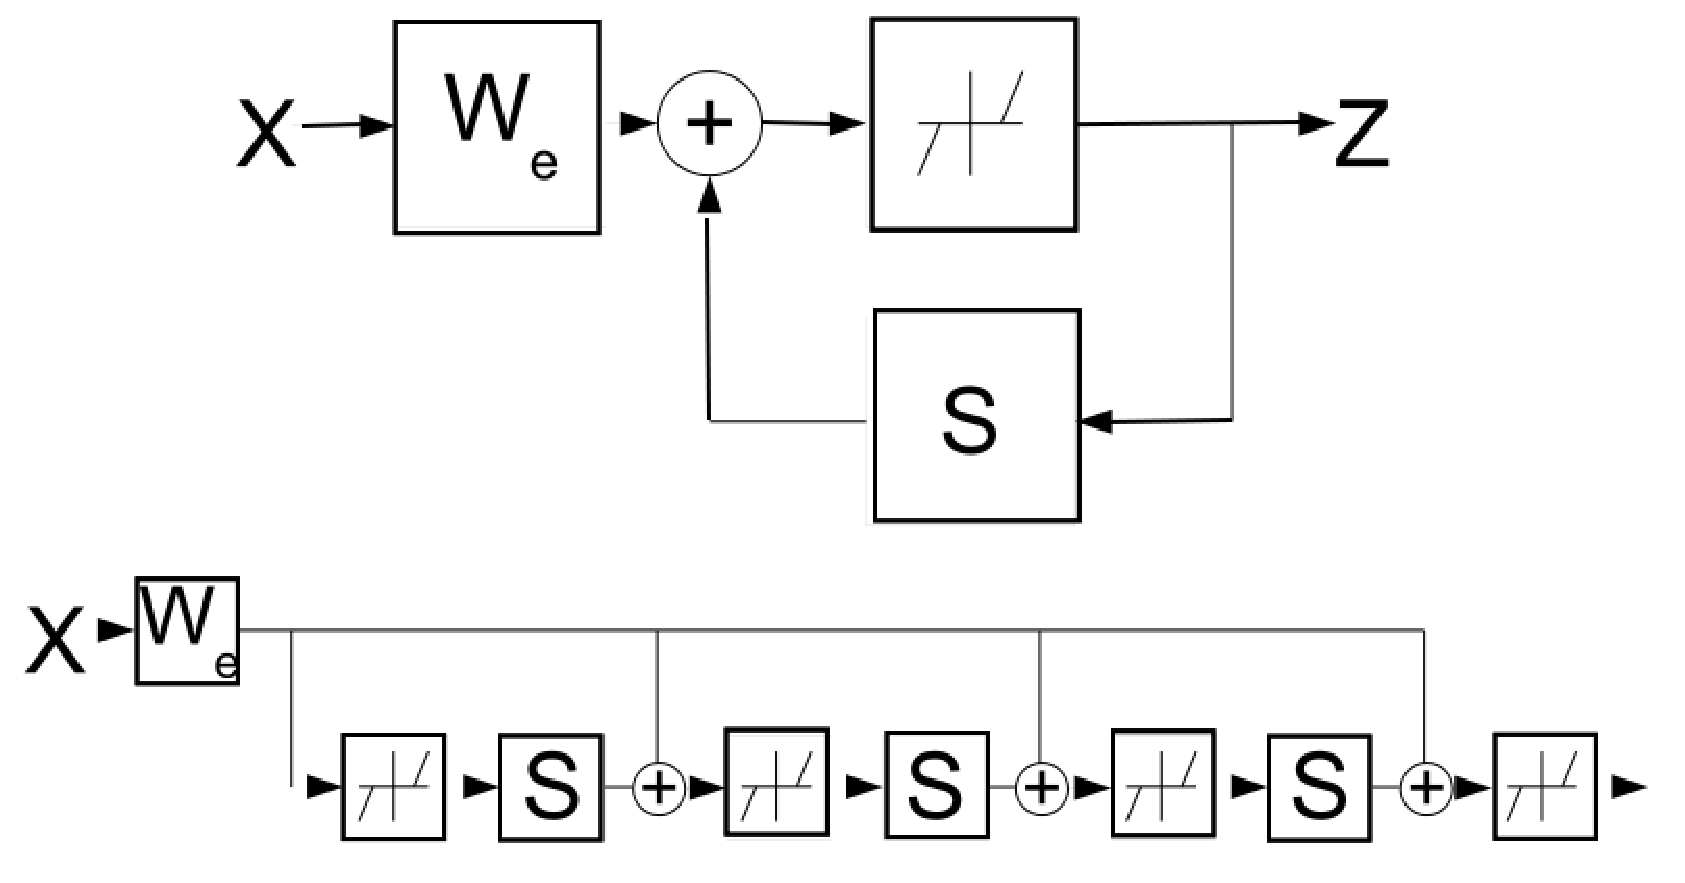
\includegraphics[scale=0.3]{./figures/LISTA/LISTA.pdf}
\caption{LISTA network architecture} 
\label{fig:LISTA} 
\end{figure}  

Recall the iterative ISTA algorithm for solving the relaxed sparse inference problem
known as the lasso was discussed in Chapter \ref{chapter:introduction}. 
The lasso loss is given by:
  
\begin{equation}
L_{lasso} = \frac{1}{2}\|X-W_dZ\| + \alpha |Z|_1 
\label{eqn:lasso} 
\end{equation} 

The LISTA network architecture is \emph{derived} by expressing the ISTA
algorithm as a recurrent network, and ``unrolling'' into a finite number of
loops with shared-weight stages.  The recurrent and unrolled networks
(three-loops) are shown in Figure \ref{fig:LISTA}. Note that
$S=I-\frac{1}{L}W_d^T W_d$, where $W_d$ is the decoder and $L$ is the upper
bound of $W_d^t W_d$. Although the ``shrinkage'' nonlinearity is depicted in
the architecture of Figure \ref{fig:LISTA}, we used rectified linear (ReLU)
non-linearities which produce non-negative sparse codes.  The above network can
be made convolutional by replacing the linear operators $W_e$ and $S$ with
convolutional filter banks. In order to be able to compute the reconstruction
error in Equation \ref{eqn:lasso}, the convolutional synthesis operator must
produce outputs of the same size as the input. This can be accomplished by
using ``same'' convolutions or by cropping the input and computing the
reconstruction error in the ``valid'' regions. As in ordinary convolutional
networks, each convolutional layer produces multiple output planes. For
example, if the encoder takes in images of 3-input planes and produces
$n$-output planes then the $S$ convolution stage takes in $n$-input planes and
produces $n$-output planes. Convolutional dictionaries are massively
overcomplete, making sparse inference a potentially much harder problem
\cite{ConvSC}. 

\section{Learning to Perform Sparse Inference} Training networks to perform
sparse inference was originally proposed in \cite{groupSparsity}, the
specialized LISTA architecture was proposed later in \cite{LISTA}. In
\cite{LISTA} networks were trained to explicitly minimize the $L^2$ distance
between the predicted and ground truth codes obtained via iterative sparse
inference.  This requires pre-training a dictionary and constructing a dataset
consisting of sparse codes corresponding to minima of the lasso loss.  However,
in \cite{groupSparsity} the networks were implicitly trained to produce sparse
codes by directly minimizing a variant of the lasso loss. The variant included
an additional term which encouraged the predicted codes to be close to the
codes which minimize the lasso loss.  In the context of dictionary learning it
is desirable to learn the encoder and decoder jointly, (i.e. training an
auto-encoder) as opposed to learning a decoder first then training an encoder
to predict the sparse codes. This section will present experimental results
which empirically answer the following questions: \begin{itemize} \item{Does
the convolutional LISTA architecture outperform other architectures when
minimizing the lasso loss with a fixed dictionary?} \item{Does the
convolutional LISTA architecture outperform other architectures when minimizing
the lasso loss with a learned dictionary?} \end{itemize} The following
experiments were performed on the whitened CIFAR-10 dataset (Figure
\ref{fig:CIFAR_rec}), all reported results were obtained on the CIFAR-10 test
set. Fixed-dictionary experiments used a pre-trained decoder obtained via
convolutional sparse coding with FISTA inference \cite{ConvSC}.  This decoder
was used to perform the fixed-dictionary experiments. The decoder consists of
32-convolutional $3\times9\times9$ filters shown in Figure
\ref{fig:FISTA_decoder}. 

The top plot of Figure \ref{fig:learning_curves} presents the learning curves
corresponding to the first five epochs of training LISTA architectures with
0,1,and 5 loops. The networks were trained to predict the sparse codes obtained
using 10-iterations of FISTA inference by directly minimizing the distance in
code space, namely:

\begin{equation} 
\nonumber 
\min_{W_e,S} \|Z_{FISTA} - LISTA_n(X;W_e,S) \|
\end{equation} 

The codes obtained with FISTA corresponding to the samples in Figure \ref{fig:CIFAR_rec}
are visualized in Figure \ref{fig:activations}. 

\begin{figure} \centering
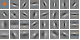
\includegraphics[scale=2]{./figures/LISTA/FISTA_decoder.png}
\caption{Pre-trained decoder used for fixed-decoder experiments}
\label{fig:FISTA_decoder} \end{figure}  

\begin{figure} 
\centering
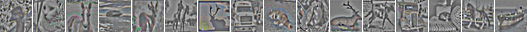
\includegraphics[scale=0.75]{./figures/LISTA/sample.png}

\includegraphics[scale=0.75]{./figures/LISTA/rec.png}
\caption{Whitened CIFAR-10 samples (top) and their corresponding reconstructions.}
\label{fig:CIFAR_rec} \end{figure}  

\begin{figure} \centering
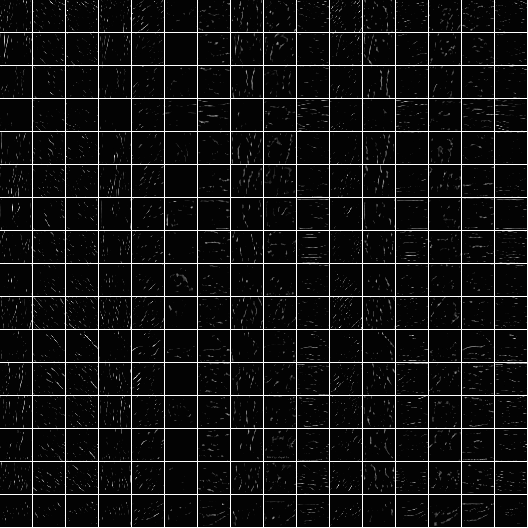
\includegraphics[scale=0.75]{./figures/LISTA/activations.png}
\caption{Sparse codes obtained with FISTA inference}
\label{fig:activations} \end{figure}  

In the above Equation $LISTA_n$ refers to a LISTA network with $n$-loops of
\emph{shared} weights. The networks are trained via stochastic gradient descent
with fixed learning rate. The top plot of Figure \ref{fig:learning_curves}
presents the learning curves corresponding to the first five epochs of training
LISTA architectures with 0,1,and 5 loops. The bottom plot tracks the loss
corresponding to the codes output by the networks at the corresponding epochs.
The loss corresponding to 10-iterations of FISTA is shown as dashed red line. 
The loss is usually, but not always, commensurate with the distance in code
space. Note that despite having the \emph{same number of trainable parameters}
LISTA networks with more loops seem to converge to a lower loss, or at least
converge faster.  However, the reason for this phenomena could be do to the
fact that networks with more loops implicitly use a larger learning rate since
gradients add in shared-weight networks. To eliminate this possibility, we use
a coarse to fine random grid search to find the optimal learning rate for each
network in the following experiments.

\begin{figure} \centering
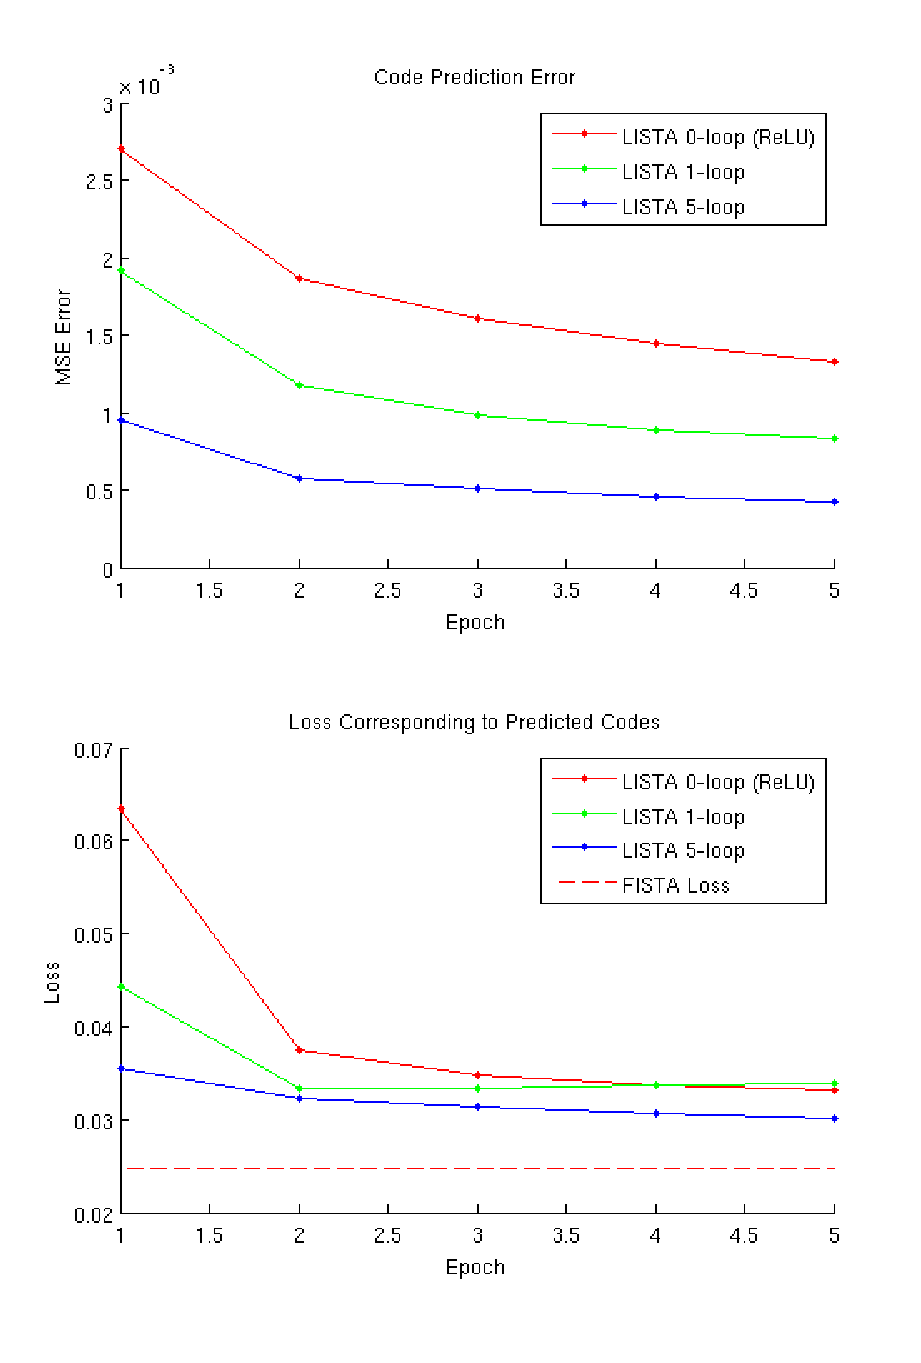
\includegraphics[scale=0.75]{./figures/LISTA/code_pred.pdf} \caption{Sparse
inference learning curves} \label{fig:learning_curves} \end{figure}  


\subsection{Sparse Inference in a Fixed Dictionary}      

\begin{figure} \centering
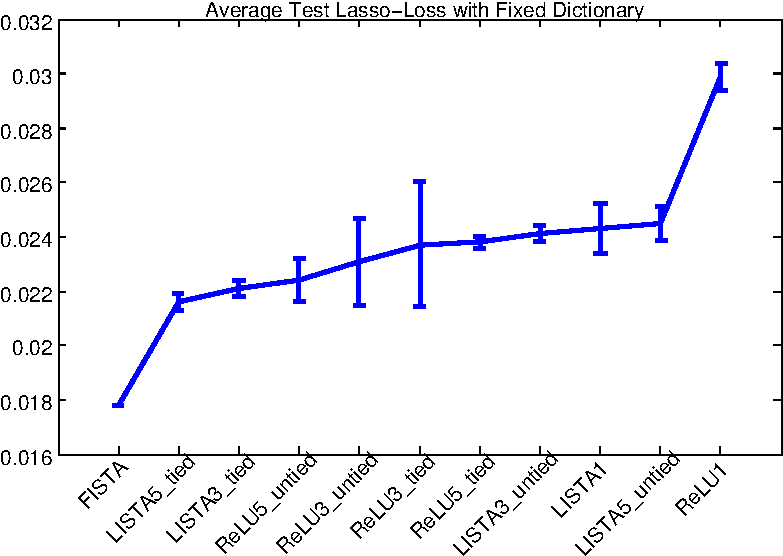
\includegraphics[scale=0.75]{./figures/LISTA/fixed_decoder_loss.pdf}
\caption{Lasso Loss} \label{fig:lasso_loss} \end{figure}  

\begin{figure} \centering
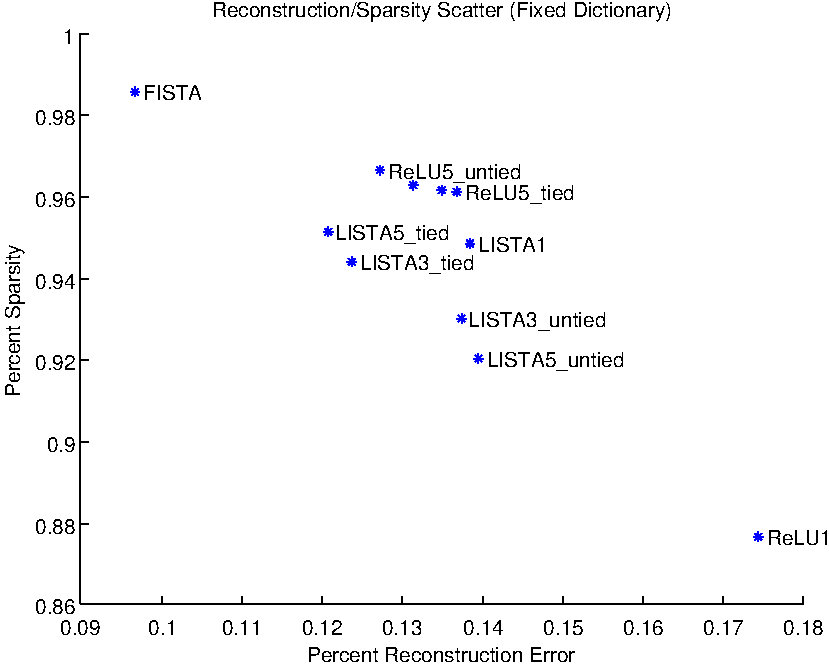
\includegraphics[scale=0.75]{./figures/LISTA/fixed_decoder_scatter.pdf}
\caption{Scatter Plot} \label{fig:scatter_fixed} \end{figure}  

The following experiments compare the performance of various architectures in
minimizing Equation \ref{eqn:lasso}, with $\alpha=0.5$. We compare the
performance of the LISTA architecture to that of a more traditional deep ReLU
networks, namely trainable convolutional layer interspersed with rectified
linear point-wise non-linearities.  Additionally we evaluate whether sharing
weights is beneficial in networks trained for sparse inference. To this end,
all multi-layer networks are trained with tied and untied weights. All
experiments were repeated five times with different random initializations in
order to measure the performance variance. Figure \ref{fig:lasso_loss}
shows the lasso test loss corresponding the codes produced by the various
architectures.  The error bars correspond to the empirical standard deviation
obtained by training each network from five different random intializations.
The loss corresponding to the FISTA iterative inference algorithm (shown on the
left side of the $x$-axis) can be considered as the lower bound on the test
set. The next best codes are produced by the LISTA network with the most loops
(five) and \emph{shared} weights. ReLU networks had identical capacity as the
LISTA networks, namely the $W_e$ and $S$ filter banks, with the skip
connections of the LISTA networks removed. Figure \ref{fig:scatter_fixed} shows
a scatter plot where each point once again corresponds to the codes produced by
each network. The $x$-axis is the average percent reconstruction error, and the
$y$-axis is the percent sparsity (proportion of activations that are zero).
From these results, it can be concluded that indeed the LISTA architecture is
superior to the ReLU network baseline. Moreover, shared weight LISTA networks
outperform their untied weight counterparts despite having a smaller capacity.       



